%%%%%%%%%%%%%%%%%%%%%%%%%%%%%%%%%%%%%%%%%%%%%%%%%%%%%%%%%%%%%%%%%%%%%%
% LaTeX Template: Curriculum Vitae
%
% Source: http://www.howtotex.com/
% Feel free to distribute this template, but please keep the
% referal to HowToTeX.com.
% Date: July 2011
% 
%%%%%%%%%%%%%%%%%%%%%%%%%%%%%%%%%%%%%%%%%%%%%%%%%%%%%%%%%%%%%%%%%%%%%%
% How to use writeLaTeX: 
%
% You edit the source code here on the left, and the preview on the
% right shows you the result within a few seconds.
%
% Bookmark this page and share the URL with your co-authors. They can
% edit at the same time!
%
% You can upload figures, bibliographies, custom classes and
% styles using the files menu.
%
% If you're new to LaTeX, the wikibook is a great place to start:
% http://en.wikibooks.org/wiki/LaTeX
%
%%%%%%%%%%%%%%%%%%%%%%%%%%%%%%%%%%%%%%%%%%%%%%%%%%%%%%%%%%%%%%%%%%%%%%
\documentclass[paper=a4,fontsize=11pt]{scrartcl} % KOMA-article class
							
\usepackage[english]{babel}
\usepackage[utf8x]{inputenc}
\usepackage[protrusion=true,expansion=true]{microtype}
\usepackage{amsmath,amsfonts,amsthm}     % Math packages
\usepackage{graphicx}                    % Enable pdflatex
\usepackage[svgnames]{xcolor}            % Colors by their 'svgnames'
\usepackage{geometry}
	\textheight=700px                    % Saving trees ;-)
\usepackage{url}

\frenchspacing              % Better looking spacings after periods
\pagestyle{empty}           % No pagenumbers/headers/footers

%%% Custom sectioning (sectsty package)
%%% ------------------------------------------------------------
\usepackage{sectsty}

\sectionfont{%			            % Change font of \section command
	\usefont{OT1}{phv}{b}{n}%		% bch-b-n: CharterBT-Bold font
	\sectionrule{0pt}{0pt}{-5pt}{3pt}}

%%% Macros
%%% ------------------------------------------------------------
\newlength{\spacebox}
\settowidth{\spacebox}{8888888888}			% Box to align text
\newcommand{\sepspace}{\vspace*{1em}}		% Vertical space macro

\newcommand{\MyName}[1]{ % Name
		\Huge \usefont{OT1}{phv}{b}{n} \hfill #1
		\par \normalsize \normalfont}
		
\newcommand{\MySlogan}[1]{ % Slogan (optional)
		\large \usefont{OT1}{phv}{m}{n}\hfill \textit{#1}
		\par \normalsize \normalfont}

\newcommand{\NewPart}[1]{\section*{\uppercase{#1}}}

\newcommand{\PersonalEntry}[2]{
		\noindent\hangindent=2em\hangafter=0 % Indentation
		\parbox{\spacebox}{        % Box to align text
		\textit{#1}}		       % Entry name (birth, address, etc.)
		\hspace{1.5em} #2 \par}    % Entry value

\newcommand{\SkillsEntry}[2]{      % Same as \PersonalEntry
		\noindent\hangindent=2em\hangafter=0 % Indentation
		\parbox{\spacebox}{        % Box to align text
		\textit{#1}}			   % Entry name (birth, address, etc.)
		\hspace{1.5em} #2 \par}    % Entry value	
		
\newcommand{\EducationEntry}[4]{
		\noindent \textbf{#1} \hfill      % Study
		\colorbox{Black}{%
			\parbox{6em}{%
			\hfill\color{White}#2}} \par  % Duration
		\noindent \textit{#3} \par        % School
		\noindent\hangindent=2em\hangafter=0 \small #4 % Description
		\normalsize \par}

\newcommand{\WorkEntry}[4]{				  % Same as \EducationEntry
		\noindent \textbf{#1} \hfill      % Jobname
		\colorbox{Black}{\color{White}#2} \par  % Duration
		\noindent \textit{#3} \par              % Company
		\noindent\hangindent=2em\hangafter=0 \small #4 % Description
		\normalsize \par}

%%% Begin Document
%%% ------------------------------------------------------------
\begin{document}
% you can upload a photo and include it here...
%\begin{wrapfigure}{l}{0.5\textwidth}
%	\vspace*{-2em}
%		\includegraphics[width=0.15\textwidth]{photo}
%\end{wrapfigure}
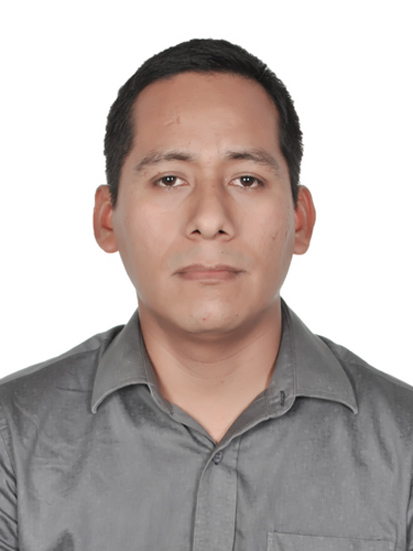
\includegraphics[width=0.2\textwidth]{Victor-Martinez.jpg}

\MyName{Victor Raúl Martinez De La Cruz}
\MySlogan{Curriculum Vitae}



%%% Personal details
%%% ------------------------------------------------------------
\NewPart{Información Personal}{}

\PersonalEntry{Nacimiento}{4 de Julio, 1987}
\PersonalEntry{Dirección}{Urb. Santa Catalina 245C, La Victoria, Lima}
\PersonalEntry{Celular}{(+51) 958-311-124 }
\PersonalEntry{Correo}{\url{devick4@gmail.com}}
\PersonalEntry{DNI}{45386831}
\PersonalEntry{Religión}{Cristiano}
\PersonalEntry{Nacionalidad}{Peruano}
\PersonalEntry{Domicilio}{Lima}
\PersonalEntry{Estado Civil} {Casado}

%%% Education
%%% ------------------------------------------------------------
\NewPart{Educación}{}

\EducationEntry{Bach. Ingeniería Electrónica}{2004-2011}{Universidad Nacional San Luis Gonzaga}{Ica}

\EducationEntry{Matriculation}{1999-2003}{Colegio Nacional San Luis Gonzaga}{5to puesto}
\newpage

%%% Work experience
%%% ------------------------------------------------------------
\NewPart{Experiencia Laboral}{}

\EducationEntry{IT Specialist}{2017-2020}{IBM del Perú}{Operador de Networking y operador de procesos batch)(Enero 2017-Actualidad) en Centro de Cómputo de Interbank(Torre Interbank)}


\EducationEntry{Administrador de Redes}{2014-2016}{Adexus Perú}{Operador de Networking, Operador de procesos batch desde 23-01-2014 hasta 31-12-2016 en Centro de Cómputo de Interbank (Torre Interbank)}

\EducationEntry{Operador de Networking}{2012-2013}{Adexus Perú}{Operador de Networking desde 01-12-2012 hasta 28-02-2013 en Proyecto Moving Datacenter Alterno de Interbank (Sede Tecnológica Camaná)}

%%% Skills
%%% ------------------------------------------------------------
\NewPart{Habilidades}{}

\SkillsEntry{Idiomas}{English}
\SkillsEntry{}{Español}

\SkillsEntry{Software de Ingeniería}{\textsc{Matlab}, \LaTeX, \textsc{Multisim}, \textsc{proteus},\textsc{workbench},\textsc{PCPIS},\textsc{Keil} }
\SkillsEntry{Software Adicional}{\textsc{Microsoft office(MS word,power point)}}
%%% Skills
%%% ------------------------------------------------------------
\NewPart{hobbies}{Trabajo en diseño web backend\\Juegos online}
%%% Skills
%%% ------------------------------------------------------------
\NewPart{Referencias}{Disponibles a solicitud }
\end{document}
